\documentclass{standalone}
\usepackage{tikz}
\usepackage{nono}
\begin{document}
  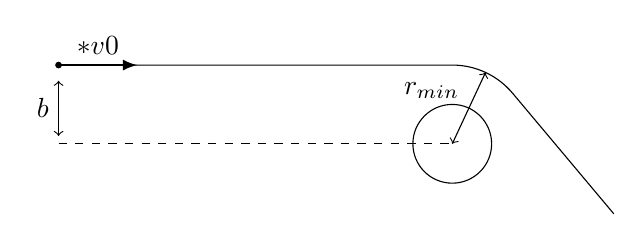
\begin{tikzpicture}
    \draw (5, 0) circle (0.5cm);
    \draw (0, 1) -- (5, 1) arc(90:40:1) -- ++(-50:2);
    \draw[<->] (5, 0) -- ++(65: 1) node[midway, above left] {$r_\text{min}$}; 
    \draw[dashed](0,0) -- (5,0);
    \draw[<->] (0, 0.1) -- (0, 0.8) node[midway, left]{$b$}; 
    \draw[fill] (0, 1) circle(1pt);
    \draw[-latex, thick] (0,1) -- ++(1,0) node[midway, above]{$\vv*{v}{0}$};
  \end{tikzpicture}
\end{document}
